\section{Experiments}
\label{sec:experiments}

\paragraph{Testbeds and protocol.} \textbf{COMPAS} is real in every respect
that matters: judges' pretrial release decisions are real, and two-year
rearrest is \emph{recorded} for detained and released defendants alike
(ProPublica's Broward County file, $n=\nCompasTarNCohort$ after the published
cohort filter and a custody-length cap; \cref{app:compas-audit}). We hide the
detained defendants' labels from every method and score against the recorded
outcome. We do not call it ground truth: detention also incapacitates, and
\cref{app:compas-audit} reports the exposure-adjusted variant.
\textbf{Lending Club} is \emph{semi-synthetic}: real applicant features and
repayment outcomes, the underwriter's own assigned interest rate and
sub-grade held out as the private signal $S$ (a real variable that predicts
default and is absent from application data; a code-level guard keeps it out
of $X$, \cref{app:lending-guard}), and a funding decision drawn from a
$\Gamma_0$-calibrated policy in $(X,S)$. \textbf{SL-Bench} is synthetic with
exact oracle quantities by quadrature and the confounding scale bisected to a
target $\Gamma_0$. A simulated emergency-department cohort only validates the
pipeline (\cref{app:simulator}); the real-data medical arm is specified in
\cref{app:medical} and its numbers are pending. Every number is out of sample with cross-fitted, isotonically
calibrated nuisances (\cref{app:nuisance-est}), averaged over
$\nExpTwoSeeds$ seeds with 95\% confidence intervals; where a CI is not
printed it is below the last digit shown.

\subsection{Real decisions: COMPAS}
\label{sec:compas}

\begin{table*}[t]
\centering\small
\caption{\textbf{Deployment metrics and certificates, out of sample}, mean
over $\nExpTwoSeeds$ seeds (full method lists, observed AUROC and 95\% CIs in
\cref{app:more-tables}). \emph{Risk} and \emph{AUROC} are on the recorded or
complete outcomes of \emph{all} units; \emph{w.c.\ risk} and \emph{regret}
are certified at the data's own odds ratio (COMPAS, $\Gamma=\nCompasOR$) or
the instance's $\Gamma_0$ (Lending $\nExpTwoLendingGammaZero$, SL-Bench
$\nExpTwoSlBenchGammaZero$). Best non-oracle value per column in bold.}
\label{tab:main}
\resizebox{\textwidth}{!}{\begin{tabular}{l cccc cccc cccc}
\toprule
& \multicolumn{4}{c}{COMPAS (real)} & \multicolumn{4}{c}{Lending Club (semi-synthetic)} & \multicolumn{4}{c}{SL-Bench (synthetic)}\\
\cmidrule(lr){2-5}\cmidrule(lr){6-9}\cmidrule(lr){10-13}
method & risk & AUROC & w.c.\ & regret & risk & AUROC & w.c.\ & regret & risk & AUROC & w.c.\ & regret\\
\midrule
ERM-observed & $\nCompasMErmRisk$ & $\nCompasMErmAuroc$ & $\nCompasMErmWc$ & $\nCompasMErmRegret$ & $\nExpTwoLendingErmRisk$ & $\nExpTwoLendingErmAuroc$ & $\nExpTwoLendingErmWc$ & $\nExpTwoLendingErmRegret$ & $\nExpTwoSlBenchErmRisk$ & $\nExpTwoSlBenchErmAuroc$ & $\nExpTwoSlBenchErmWc$ & $\nExpTwoSlBenchErmRegret$\\
AIPW & $\nCompasMAipwRisk$ & $\nCompasMAipwAuroc$ & $\nCompasMAipwWc$ & $\nCompasMAipwRegret$ & $\nExpTwoLendingAipwRisk$ & $\nExpTwoLendingAipwAuroc$ & $\nExpTwoLendingAipwWc$ & $\nExpTwoLendingAipwRegret$ & $\nExpTwoSlBenchAipwRisk$ & $\nExpTwoSlBenchAipwAuroc$ & $\nExpTwoSlBenchAipwWc$ & $\nExpTwoSlBenchAipwRegret$\\
Heckman probit & $\mathbf{\nCompasMHeckmanRisk}$ & $\mathbf{\nCompasMHeckmanAuroc}$ & $\nCompasMHeckmanWc$ & $\nCompasMHeckmanRegret$ & $\nExpTwoLendingHeckmanRisk$ & $\mathbf{\nExpTwoLendingHeckmanAuroc}$ & $\nExpTwoLendingHeckmanWc$ & $\nExpTwoLendingHeckmanRegret$ & $\mathbf{\nExpTwoSlBenchHeckmanRisk}$ & $\mathbf{\nExpTwoSlBenchHeckmanAuroc}$ & $\nExpTwoSlBenchHeckmanWc$ & $\nExpTwoSlBenchHeckmanRegret$\\
Manski ($\Gamma=\infty$) & $\nCompasMManskiRisk$ & $\nCompasMManskiAuroc$ & $\nCompasMManskiWc$ & $\nCompasMManskiRegret$ & $\nExpTwoLendingManskiRisk$ & $\nExpTwoLendingManskiAuroc$ & $\nExpTwoLendingManskiWc$ & $\nExpTwoLendingManskiRegret$ & $\nExpTwoSlBenchManskiRisk$ & $\nExpTwoSlBenchManskiAuroc$ & $\nExpTwoSlBenchManskiWc$ & $\nExpTwoSlBenchManskiRegret$\\
DCL, minimax risk & $\nCompasMDclTwoRisk$ & $\nCompasMDclTwoAuroc$ & $\mathbf{\nCompasMDclTwoWc}$ & $\nCompasMDclTwoRegret$ & $\mathbf{\nExpTwoLendingDclTwoRisk}$ & $\nExpTwoLendingDclTwoAuroc$ & $\mathbf{\nExpTwoLendingDclTwoWc}$ & $\nExpTwoLendingDclTwoRegret$ & $\nExpTwoSlBenchDclThreeRisk$ & $\nExpTwoSlBenchDclThreeAuroc$ & $\mathbf{\nExpTwoSlBenchDclThreeWc}$ & $\nExpTwoSlBenchDclThreeRegret$\\
DCL, minimax regret & $\nCompasMDclRegTwoRisk$ & $\nCompasMDclRegTwoAuroc$ & $\nCompasMDclRegTwoWc$ & $\mathbf{\nCompasMDclRegTwoRegret}$ & $\nExpTwoLendingDclRegTwoRisk$ & $\nExpTwoLendingDclRegTwoAuroc$ & $\nExpTwoLendingDclRegTwoWc$ & $\mathbf{\nExpTwoLendingDclRegTwoRegret}$ & $\nExpTwoSlBenchDclRegThreeRisk$ & $\nExpTwoSlBenchDclRegThreeAuroc$ & $\nExpTwoSlBenchDclRegThreeWc$ & $\mathbf{\nExpTwoSlBenchDclRegThreeRegret}$\\
\emph{oracle (uncensored)} & \emph{$\nCompasMOracleRisk$} & \emph{$\nCompasMOracleAuroc$} & \emph{$\nCompasMOracleWc$} & \emph{$\nCompasMOracleRegret$} & \emph{$\nExpTwoLendingOracleRisk$} & \emph{$\nExpTwoLendingOracleAuroc$} & \emph{$\nExpTwoLendingOracleWc$} & \emph{$\nExpTwoLendingOracleRegret$} & \emph{$\nExpTwoSlBenchOracleRisk$} & \emph{$\nExpTwoSlBenchOracleAuroc$} & \emph{$\nExpTwoSlBenchOracleWc$} & \emph{$\nExpTwoSlBenchOracleRegret$}\\
\bottomrule
\end{tabular}}
\end{table*}

\begin{figure}[t]
\centering
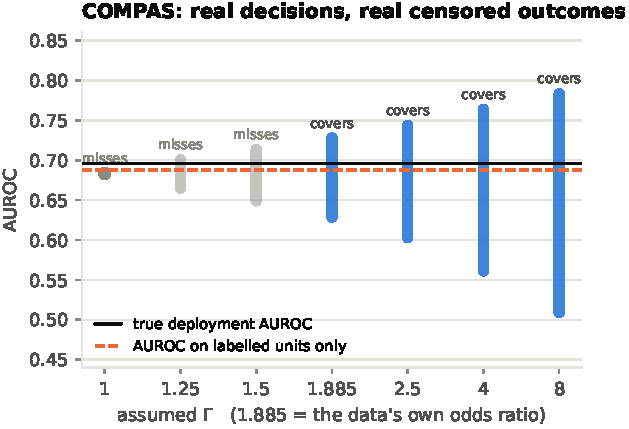
\includegraphics[width=0.5\linewidth]{figures/fig2_compas}
\caption{\textbf{Real pretrial release decisions with recorded censored
outcomes.} Intervals that contain the recorded deployment AUROC are drawn in
colour, those that miss it in grey. Assuming missing-at-random ($\Gamma=1$)
collapses the interval to a point that misses; coverage begins at the $\Gamma$
implied by the data's own detained-versus-released odds ratio,
$\nCompasOR$.}
\label{fig:compas}
\end{figure}

\Cref{fig:compas} checks the bounds against decisions no one simulated. The
recorded odds ratio between the detained and released groups' rearrest rates
is $\nCompasOR$. At $\Gamma=1$ --- the missing-at-random assumption that IPW
and AIPW require --- the interval collapses to a point and covers the recorded
AUROC in $\nCompasCovAtOne$ of splits. Coverage reaches $\nCompasCovAtOR$ at
$\Gamma=\nCompasOR$, where the interval has width $\nCompasWidthAtOR$: narrow
enough to be useful, wide enough to be honest. Corner evaluation covers in
$\nCompasCornerCovAtOR$ of splits at that $\Gamma$. Holding time at risk fixed
(\cref{app:compas-audit}) \emph{raises} the odds ratio to $\nCompasExpOR$ ---
incapacitation was masking selection, not creating it --- and coverage at that
anchor is $\nCompasExpCovAtOR$. \Cref{tab:main} repeats the method
comparison. The minimax-regret rule certifies a regret
$\nCompasRegretRatioErm\times$ tighter than ERM while its realised risk
($\nCompasMDclRegTwoRisk$) is lower than every baseline's except the
parametric selection model's, and lower than the \emph{oracle}'s
($\nCompasMOracleRisk$); Heckman's realised risk is also the least stable
across splits ($\nCompasMHeckmanRiskMin$--$\nCompasMHeckmanRiskMax$), as one
expects of identification that rests on a functional form. We read this as
the strongest available evidence that $\dcsm(\Gamma)$, with $\Gamma$ anchored
to leniency or odds-ratio structure, is the right object to report.



\subsection{The bounds are sharp, valid and cheap}
\label{sec:exp-sharp}

\begin{table}[t]
\centering\small
\caption{\textbf{Sharpness and validity of the AUROC interval} (SL-Bench,
$\nExpOneNCells$ cells of $(\Gamma_0,\Gamma)$ over $\Gamma_0\in\{1.5,2,3,5\}$,
$\Gamma\in\{1,\dots,8\}$, $\nExpOneSeeds$ seeds). Coverage is of the true
\emph{deployment} AUROC on held-out units. Corner evaluation is narrow because
it is wrong.}
\label{tab:sharpness}
\resizebox{\linewidth}{!}{\begin{tabular}{lccc}
\toprule
 & sharp (\cref{thm:sharp-auc}) & separate bounds & corner evaluation \\
\midrule
coverage when $\Gamma\ge\Gamma_0$ & $\mathbf{\nExpOneCovSharp}$ & $\nExpOneCovSeparate$ & $\nExpOneCovCorner$ \\
mean interval width               & $\nExpOneWidthSharp\pm\nExpOneWidthSharpCI$ & $\nExpOneWidthSeparate$ & $\nExpOneWidthCorner$ \\
coverage when $\Gamma<\Gamma_0$   & $\nExpOneCovTooSmall$ & --- & --- \\
\midrule
max $|$analytic $-$ brute force$|$ & \multicolumn{3}{c}{$\nExpOneGap$}\\
max $|\AUC(p^\star)-\text{bound}|$ (attainment) & \multicolumn{3}{c}{$\nExpOneAttain$}\\
runtime, $n=20{,}000$ / $100{,}000$ / $400{,}000$ & \multicolumn{3}{c}{$\nExpOneRuntimeTwentyK$s / $\nExpOneRuntimeHundredK$s / $\nExpOneRuntimeFourHundredK$s}\\
\bottomrule
\end{tabular}}
\end{table}

\Cref{tab:sharpness} tests \cref{thm:sharp-auc} three ways. \emph{Sharpness}:
an independent projected-gradient search over the identified box never escapes
the analytic interval and matches it to $\nExpOneGap$, while the extremal
$p^\star$ returned by the theorem lies in the box and attains the bound to
machine precision. \emph{Validity}: whenever $\Gamma\ge\Gamma_0$ the sharp
interval covers the deployment AUROC in $\nExpOneCovSharp$ of cells, degrading
to $\nExpOneCovTooSmall$ --- gracefully, not catastrophically --- when the
assumed $\Gamma$ is too small (\cref{app:misspec}). Corner evaluation covers in
$\nExpOneCovCorner$ of cells: it is $\nExpOneWidthRatioCorner\times$ narrower
than the sharp interval and, as \cref{prop:corner} predicts and
\cref{app:counterexample} exhibits, narrow for the wrong reason. Bounding
numerator and denominator separately is valid but
$\nExpOneWidthRatioSep\times$ wider, which is what sharpness buys.
\emph{Cost}: $400{,}000$ units in $\nExpOneRuntimeFourHundredK$ seconds.

\subsection{Decision-censored learning}
\label{sec:exp-learning}



\Cref{tab:main} (and \cref{fig:learning} in \cref{app:more-tables}) puts \cref{thm:dcl} and
\cref{prop:regret} against the field. \emph{The certificates.} DCL attains the
best worst-case risk on every testbed by construction; the margin is what
matters: $\nExpTwoLendingWcRatioErmOverDcl\times$ against ERM on Lending Club.
Certified regret separates the methods more sharply: the minimax-regret rule
\eqref{eq:regret-rule} cuts it by $\nExpTwoLendingRegretRatioErm\times$ against
ERM on Lending Club and $\nExpTwoSlBenchRegretRatioErm\times$ on SL-Bench.
The \emph{oracle}, fit on the uncensored labels, has poor certified regret: it
is tuned to one member of the identified set and is not robust to the others.
\emph{The realised metrics.} On Lending Club the two DCL rules also have the
lowest realised risk of any method, the oracle and the parametric selection
model included, and on COMPAS the minimax-regret rule is below every
baseline but Heckman and below the oracle --- not because they know more, but
because shrinking a calibrated estimate toward the decision boundary is a
better-conditioned estimator than fitting flexibly to labels. On SL-Bench, where the Heckman model's normality
assumption holds by construction, the parametric selection model attains the
best realised risk and DCL pays a small price for not assuming a functional
form. The minimax-\emph{risk} rule is uniformly more conservative; Manski
($\Gamma=\infty$) is valid and useless, with realised risk
$\nExpTwoLendingManskiRiskRatioErm\times$ ERM's on Lending Club.
\emph{The blind spot.} The observed AUROC differs from the deployment AUROC by
$\nExpTwoLendingErmObsMinusTrue$ on Lending Club and
$\nExpTwoSlBenchErmObsMinusTrue$ on SL-Bench; the sign differs between
testbeds, which is precisely why a sensitivity analysis is needed to know it.



\subsection{Falsifying $\Gamma$, break-even, generalisation and uncertainty}
\label{sec:exp-rest}

\begin{table}[t]
\centering\small
\caption{\textbf{Falsifying $\Gamma$ from leniency variation} (SL-Bench, 5
decision makers, 30 configurations). $\Gamma_0^{\mathrm{cond}}$ is the
\emph{within-decision-maker} sensitivity parameter, which is what
\cref{prop:falsify} bounds from below. ``Recovered'' is
$\log\Gamma_{\min}/\log\Gamma_0^{\mathrm{cond}}$ at the robust ($95$th
percentile) variant. The bound was valid in every one of the 30 cells, and never
refuted a true missing-at-random mechanism.}
\label{tab:falsify}
\begin{tabular}{cccccc}
\toprule
target $\Gamma_0$ & reliance on $S$ & $\Gamma_0^{\mathrm{cond}}$ &
$\Gamma_{\min}$ & $\Gamma_{\min}$ (q95) & recovered\\
\midrule
$1.0$ & homogeneous   & $1.000$  & $1.000$ & $1.000$ & --- \\
$1.0$ & heterogeneous & $1.000$  & $1.000$ & $1.000$ & --- \\
$1.5$ & homogeneous   & $1.582$  & $1.423$ & $1.341$ & $0.61$\\
$1.5$ & heterogeneous & $1.862$  & $1.573$ & $1.398$ & $0.51$\\
$2.0$ & homogeneous   & $2.273$  & $1.814$ & $1.594$ & $0.54$\\
$2.0$ & heterogeneous & $2.924$  & $2.181$ & $1.685$ & $0.45$\\
$3.0$ & homogeneous   & $3.831$  & $2.409$ & $1.914$ & $0.45$\\
$3.0$ & heterogeneous & $5.445$  & $3.164$ & $2.047$ & $0.39$\\
$5.0$ & homogeneous   & $7.623$  & $3.171$ & $2.270$ & $0.37$\\
$5.0$ & heterogeneous & $11.195$ & $4.420$ & $2.419$ & $0.34$\\
\bottomrule
\end{tabular}
\end{table}

\paragraph{The test never over-claims, and never cries wolf.}
\Cref{tab:falsify} reports $\Gamma_{\min}$ across 30 configurations varying the
true $\Gamma_0$, the spread of leniency, and whether decision makers rely on
their private information to the same degree. Two properties hold without
exception. First, \emph{validity}: $\Gamma_{\min}\le\Gamma_0^{\mathrm{cond}}$ in
every cell, as \cref{prop:falsify} requires. Second, \emph{no false alarms}: when
the mechanism really is missing-at-random the test returns exactly $1.000$ and
refutes nothing, so an analyst who runs it on genuinely unconfounded data is not
pushed into a needless sensitivity analysis.

\paragraph{How much it recovers.} \Cref{fig:falsify} plots every configuration
against the truth; on the log scale the test recovers $34$--$61\%$
of the truth, and --- as theory predicts --- less when decision makers differ in
\emph{how much} they use their private information rather than only in how
lenient they are: heterogeneity in reliance is exactly what makes different
decision makers' identified sets overlap for smaller $\Gamma$. So
$\Gamma_{\min}$ should be read as what it is: a floor the data will not let you
go below, not an estimate of $\Gamma_0$. At $\Gamma_0=3$ it already refutes
$\dcsm(\Gamma)$ for every $\Gamma<1.9$, which rules out missing-at-random ---
and with it IPW and AIPW --- decisively.

\begin{figure}[t]
\centering
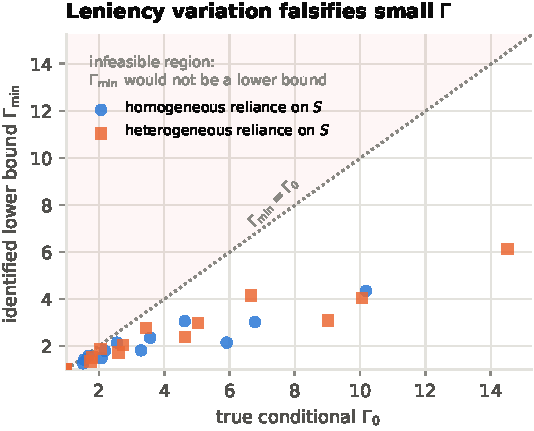
\includegraphics[width=0.58\linewidth]{figures/fig6_falsification}
\caption{\textbf{Every point lies below the diagonal:} the identified lower bound
never exceeds the true conditional $\Gamma_0$. Heterogeneous reliance on private
information across decision makers loosens the bound, as \cref{prop:falsify}'s
intersection argument predicts.}
\label{fig:falsify}
\end{figure}

\paragraph{Break-even analysis: what survives.}
The deliverable a practitioner wants is not a single interval but the $\Gamma$ at
which a conclusion flips. On Lending Club the incumbent model's AUROC lower bound
stays above $0.55$ up to $\Gamma=1.72$ and above chance up to $\Gamma=2.82$ ---
so the claim ``this model ranks better than chance'' survives past the true
$\Gamma_0=2.0$, while the stronger claim ``AUROC is at least $0.60$'' does not
survive even $\Gamma=1.05$. On MIMIC-sim, where the model is far more
discriminative, the above-chance claim survives to $\Gamma=14.9$. Separately, the
DCL model's certified worst-case risk beats the incumbent's at \emph{every}
$\Gamma$ we tested, up to $\Gamma=40$: the ordering of models under the
certificate is robust even where the absolute numbers are not.

\paragraph{When $\Gamma$ is set too small.} \Cref{tab:misspec} shows the failure
mode is graceful. Coverage is $100\%$ for every $\Gamma$ at least half the truth
and falls only to $69\%$ at $\Gamma\le\Gamma_0/2$, while the interval widens
monotonically and slowly --- from $0.04$ to $0.40$ over a $200$-fold range of
$\Gamma$. The price of a conservative $\Gamma$ is a wider interval, not a wrong
one; the price of an aggressive one is a graded loss of coverage, not a cliff.

\begin{table}[t]
\centering\small
\caption{\textbf{Coverage and width when the assumed $\Gamma$ is wrong}
(SL-Bench, 3 seeds, $\Gamma$ swept over a $200$-fold range).}
\label{tab:misspec}
\begin{tabular}{lcccccc}
\toprule
$\Gamma/\Gamma_0$ & $\le 0.5$ & $(0.5, 0.8]$ & $(0.8,1.0]$ & $(1.0,1.5]$ & $(1.5,3]$ & $>3$\\
\midrule
coverage & $0.69$ & $1.00$ & $1.00$ & $1.00$ & $1.00$ & $1.00$\\
mean width & $0.04$ & $0.14$ & $0.21$ & $0.26$ & $0.35$ & $0.40$\\
\bottomrule
\end{tabular}
\end{table}

\paragraph{Generalisation.} \Cref{thm:generalization} controls the uniform
deviation over the score class. On SL-Bench (\cref{app:scaling}) it decays with
exponent $\nExpFiveDevRate$ against the $-\tfrac12$ the bound predicts, every
cell in $[\nExpFiveRateMin,\nExpFiveRateMax]$. Regressing the fitted
$n^{-1/2}$ coefficient on $\log\Gamma$ gives $R^{2}=\nExpFiveRtwoLog$; on
$\Gamma$, $R^{2}=\nExpFiveRtwoLin$. Over a $\nExpFiveGammaRange$-fold range of
$\Gamma$ the coefficient grows by $\nExpFiveCoefGrowthPct\%$ --- consistent
with the $\log\Gamma$ of \cref{cor:loggamma} and not with a linear dependence,
which would predict more than an order of magnitude. The \emph{excess risk of
the empirical minimiser} decays much faster (exponent $\nExpFiveExcessRate$):
the familiar fast-rate phenomenon for a strongly convex objective, consistent
with an upper bound without being evidence for its rate, which is why we
measure the uniform deviation instead.

\paragraph{Uncertainty.} \Cref{fig:uq} and \cref{app:uq-table} separate three
things. \emph{Identification.} With oracle nuisances every claim of
\cref{cor:uq} holds: $p_1(x)$ lies inside the identified set for
$\nExpThreeOracleInBox$ of units at every $n$, and the naive aleatoric
estimate overstates the truth by $\nExpThreeAleaBias$ nats (about
$\nExpThreeAleaBiasRelPct\%$) while sitting inside the identified interval,
where no test on observed data can refute it. \emph{Asymptotic
overconfidence.} For a converged ensemble the reported epistemic term falls by
$\nExpThreeEpiDrop\times$ between $n=2{,}000$ and $n=70{,}000$ (fitted exponent
$\nExpThreeSlopeLog$), while the censoring term moves by
$\nExpThreeCensChangePct$ with no trend; at the largest sample the ratio is
$\nExpThreeRatioLast$: the reported uncertainty is two orders of magnitude
smaller than the identification uncertainty it omits. \emph{A
different, detectable pathology.} A fixed-budget deep ensemble's ``epistemic''
term does not contract (exponent $\nExpThreeSlopeMlp$) and exceeds the
censoring term throughout, but that is optimisation noise: its calibration
error is $\nExpThreeCalRatioMlpOverLog\times$ larger, and a calibration check
catches it, unlike the bias of \cref{cor:uq}.

\begin{figure}[t]
\centering
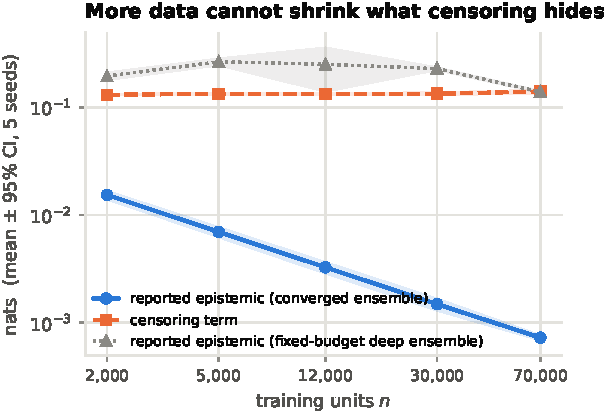
\includegraphics[width=0.58\linewidth]{figures/fig4_uq}
\caption{\textbf{More data cannot shrink what censoring hides}
(\cref{cor:uq}; $\nExpThreeSeeds$ seeds, 95\% bands). The reported epistemic
term of a converged ensemble collapses; the censoring term \eqref{eq:cens}
does not. A fixed-budget deep ensemble's term does not collapse either, for an
unrelated reason --- optimisation noise --- which a calibration check detects.}
\label{fig:uq}
\end{figure}

